\section{Multivariate optimization}
\label{sec:mvaoptimization}
% ---- ---- ---- ---- ---- ---- ---- ---- ---- ---- ---- ---- ---- ---- ---- ---- ---- ---- ---- ---- ---- ---- ----

In addition to the common preselections listed in Sec.~\ref{sec:firstStep}, the
MVA likelihood analysis applies the following selections:

\begin{itemize}
\item $|\Delta\phi_{\textrm{leading jet,MET}}| > 0.4$ for muons
\item $|\Delta\phi_{\textrm{leading jet,MET}}| > 0.8$ for electrons
\end{itemize}

For previous analyses of partial 2012 datasets we had adopted the
optimization performed on 2011 (7~TeV) data and MC samples for masses
170-600~\GeV.  That optimization was documented completely in the
analysis notes AN-2011/110 and AN-2012/008. For this analysis, we
re-optimized using the full 2012 (8~TeV) dataset and MC samples. For
this re-optimization, the basis of variable selection is unchanged;
therefore all of the input variables were kept identical. The list of
inputs are as follows:
\begin{equation}
\{ \cos\theta_1, \cos\theta_2, \Phi, \cos\theta^{\ast}, \Phi_1, p_{T,WW}, Y_{WW}, {\rm lepton~charge}\}
\end{equation}
where the angular variables are correlated and defined in
Fig.~\ref{fig:anglesWWlvjj}. We include MVA input and output parameter
plots and correlation plots for representative mass points in
Appendices~\ref{app:mvainputs}--\ref{app:mvacorr}.

%% For masses above 600~\GeV,
%% we use 8~\TeV signal samples, splitting them in half so that the half that
%% is used for training is statistically independent from the half that is
%% used for limit setting.

%% An additional point of distinction between the optimization procedures
%% for the 2011 data and this year's data is the use of the quark-gluon
%% likelihood discriminant. In 2011, this discriminant was used to
%% distinguish quark-originated jets (signal) from gluon-originated jets
%% (W+Jets dominant background), particularly at high mass ($M_{H}\geq
%% 500$~GeV), after applying the MVA output requirement. However, the PDF
%% for the discriminant for 2012 beam conditions was not yet available as
%% of this writing, and the PDF based on 2011 beam conditions did not
%% yield reliable results, so it is not applied.

\subsection{Selecting cut values}
\label{sec:mvacuts}

To select the most appropriate cut value for the new likelihood we
looked at the expected limits as a function of cut value.  It should
be noted that because of the nature of the the likelihood as
discriminator, that the value of 0.5 is the boundary between
signal-like and background-like.  In Fig.~\ref{fig:cutscan}, you can
see a representative plot for the scan, in this case for the 250~GeV
mass hypothesis.  The minimum is very broad and in almost all cases
very near to 0.5.  We adopt a cut of 0.5 for all mass-hypotheses up to
550~GeV.  For the masses 550~GeV and 600~GeV the cut is slightly
tighter at 0.6.

\begin{figure}[btph]
  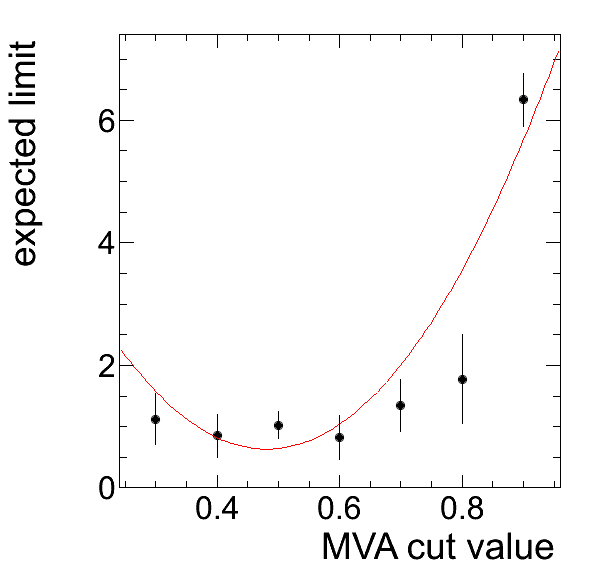
\includegraphics[width=0.48\textwidth]{plots/HWW250_mu_plot.png}
  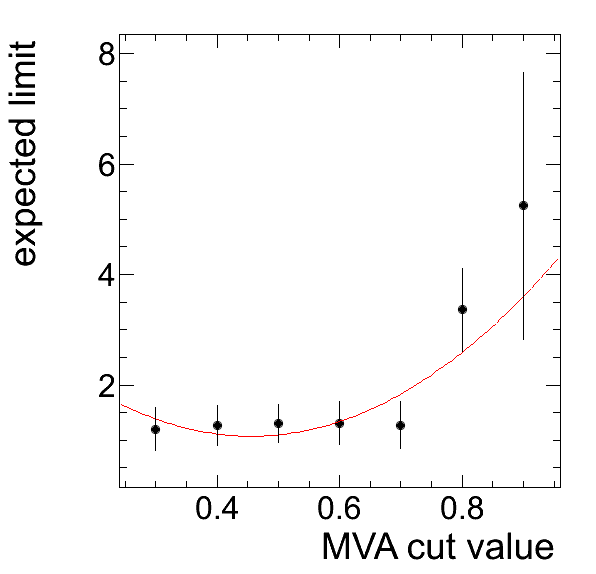
\includegraphics[width=0.48\textwidth]{plots/HWW250_el_plot.png}
  \caption{\label{fig:cutscan}Expected limit as a function of MVA cut
    value for the mass hypothesis 250~GeV.  Left is muons; right is
    electrons.}
\end{figure}
